% !TEX encoding = UTF-8 Unicode
\documentclass[11pt, a4paper, titlepage, portuguese]{article}
\usepackage[]{geometry}
	\geometry{
		a4paper,
		includehead,
		includefoot,
		top=1.7cm,
		bottom=1.7cm,
		left=2.5cm,
		right=2.5cm
	}
\usepackage[portuguese]{babel}
\usepackage[T1]{fontenc} % LaTeX
\usepackage[utf8]{inputenc} % LaTeX
\usepackage[square,sort,comma,numbers]{natbib}
\usepackage{url}
\usepackage{amsmath}
\usepackage{graphicx}
	\graphicspath{{images/}}
\usepackage{float}
\usepackage{subfig}
\usepackage[font=footnotesize]{caption}
\usepackage{vmargin}
\usepackage{enumitem}
\usepackage[document]{ragged2e}
\usepackage{tikz}
\usepackage{mwe}
\usepackage{hyperref}

\hypersetup{
    colorlinks=true,
    linkcolor=black,
    filecolor=black,     
    urlcolor=blue,
}
\urlstyle{same}

%Unidades SI
\usepackage[seperr]{siunitx}
\usepackage{mathtools}
\usepackage{setspace}
\usepackage{xcolor}
\usepackage{titlesec}
\usepackage{parskip}
\usepackage{subfig}



%\usepackage{fontspec} % XeLaTeX
\usepackage[T1]{fontenc} % LaTeX
\usepackage[utf8]{inputenc} % LaTeX
%\usepackage{newtxmath, newtxtext}
\usepackage{csquotes}
\usepackage{babel}
%\usepackage[backend=bibtex]{biblatex}
%\usepackage[backend=biber]{biblatex}
%\addbibresource{bibliography.bib}

\usepackage{indentfirst}
\usepackage{graphicx}
	\graphicspath{{images/}}
\usepackage{grffile}
\usepackage{float}
\usepackage{amsmath}
	\allowdisplaybreaks
\usepackage{physics}
\usepackage{siunitx}
	\sisetup{inter-unit-product =\ensuremath{.}}
\usepackage{hyperref}

% Section styles
%\renewcommand{\thesection}{\Roman{section}}
%\renewcommand{\thesubsection}{\alph{subsection})}
%\renewcommand{\thesubsubsection}{\roman{subsubsection}.}
\renewcommand{\thesection}{}
\renewcommand{\thesubsection}{}
\renewcommand{\thesubsubsection}{}

\titleformat*{\section}{\bfseries\vspace{12pt}\fontsize{14}{6}\rmfamily}

\titleformat*{\subsection}{\bfseries\vspace{12pt}\fontsize{14}{6}\rmfamily}

% Useful commands
\newcommand{\eq}{\Leftrightarrow} % Equivalente
% Ordem de grandeza, e.g., "2\og{5}" => "2e5"
\newcommand{\og}[1]{{\times \num{e#1}}}
% Para numerar apenas uma equação
\newcommand\numberthis{\addtocounter{equation}{1}\tag{\theequation}}

% Header and footer
\usepackage{fancyhdr}
\pagestyle{fancy}
\fancyhf{}
\lhead{Electrotecnia Teórica}
\rhead{1º Laboratório}
\lfoot{IST - Engenharia Eletrotécnica e de Computadores}
\rfoot{Página \thepage}
\renewcommand{\headrulewidth}{1pt}
\renewcommand{\footrulewidth}{0.5pt}

% Document
\begin{document}
	\begin{titlepage}
		\center
		\textsc{\bfseries\LARGE Instituto Superior Técnico}\\[1cm] % Name of your university/college
		
\includegraphics[height=1.5cm]{IST_Logo.pdf}\\[2.5cm]

		\textsc{\large Engenharia Eletrotécnica e de Computadores}\\[0.5cm] % Major heading such as course name
		\textsc{\Large Eletrotecnia Teórica}\\[0.5cm] % Minor heading such as course title
		\textsc{\large 2017/2018 2º Semestre}\\[2cm]

		\rule{\textwidth}{1.6pt}\vspace*{-\baselineskip}\vspace*{2pt} % Thick horizontal line
		\rule{\textwidth}{0.4pt}\\[\baselineskip] % Thin horizontal line
			\textsc{\Huge \bfseries 3º Trabalho Laboratorial}\\[0.2cm]
			\bigskip
			\textsc{\large \bfseries Circuito RLC série em regime forçado alternado sinusoidal}\\[0.2cm]
		\rule{\textwidth}{0.4pt}\vspace*{-\baselineskip}\vspace{3.2pt} % Thin horizontal line
		\rule{\textwidth}{1.6pt}\\[5cm]

		\begin{minipage}{0.9\textwidth}
			\begin{flushleft} \large
				\begin{Large}\bfseries\textsc{Autores:}\end{Large}\\[0.4cm]
				\begin{tabular}{l l l}
					Ricardo Simões	& 70389 & \normalsize ricardo.f.d.simoes@ist.utl.pt \\
					Rita Ramos		& 81616 & \normalsize rita.ramos@tecnico.ulisboa.pt \\
					João Pinheiro		& 84086 & \normalsize joao.castro.pinheiro@tecnico.ulisboa.pt \\
					João Sebastião		& 84087 & \normalsize joaofpsebastiao@tecnico.ulisboa.pt \\
				\end{tabular}
			\end{flushleft}
		\end{minipage}\\[0.5cm]

		\large \bfseries Laboratório segunda-feira, 09h30-11h30, Grupo D\\
		\large 30 de abril de 2018\\[1cm]
		\setcounter{page}{0}
	\end{titlepage}
	%\tableofcontents \newpage

	\section{1. Dimensionamento}
	\subsection{1.1}
	
		\begin{figure}[h]
			\centering
			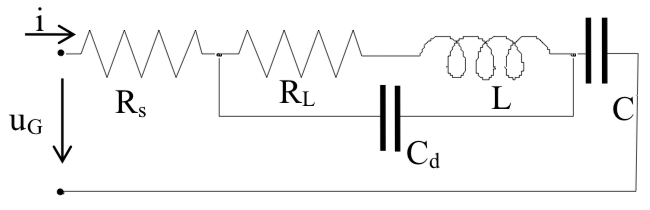
\includegraphics[width=0.6\linewidth]{circuito2.png}
			\caption{Circuito RLC tendo em conta a resistência e capacidade distribuídas na bobina}
			\label{circuito2}
		\end{figure}
	
		Pela análise do circuito da figura \ref{circuito2}, a expressão da impedância é dada por
		
		\begin{equation}
			\bar{Z} = \bar{Z}_{R_S} + \bar{Z}_{\parallel} + \bar{Z}_C,
		\end{equation}
		
		onde
		
		\begin{equation}
			\bar{Z}_{\parallel} = (\bar{Z}_{R_L} + \bar{Z}_{L}) \parallel \bar{Z}_{C_d} = \dfrac{\left(R_L + \mathrm{j} \omega L\right)\left(\dfrac{1}{\mathrm{j} \omega C_d}\right)}{(R_L + \mathrm{j} \omega L) + \dfrac{1}{\mathrm{j} \omega C_d}}.
		\end{equation}
		
		Supondo que $R_L \ll \omega L$, tem-se
		
		\begin{align}
			\bar{Z} &= R_S + \dfrac{\left(R_L + \mathrm{j} \omega L\right)\left(\dfrac{1}{\mathrm{j} \omega C_d}\right)}{R_L + \mathrm{j} \omega L + \dfrac{1}{\mathrm{j} \omega C_d}} + \dfrac{1}{\mathrm{j} \omega C} \nonumber \\
			&= R_S + \dfrac{1}{\mathrm{j} \omega C} + \dfrac{\left(\dfrac{R_L}{\omega L} + \mathrm{j}\right)\left(\dfrac{1}{\mathrm{j} \omega C_d}\right)}{\dfrac{R_L}{\omega L} + \mathrm{j} + \dfrac{1}{\mathrm{j} \omega^2 C_d L}} \nonumber \\
			&\approx R_S + \dfrac{1}{\mathrm{j} \omega C} + \dfrac{\dfrac{1}{\omega C_d}}{\mathrm{j} + \dfrac{1}{\mathrm{j} \omega^2 C_d L}} \nonumber \\
			&= R_S + \dfrac{1}{\mathrm{j} \omega C} + -\mathrm{j}\dfrac{1}{\omega C_d - \dfrac{1}{\omega L}} \nonumber \\
			&= R_S + -\mathrm{j}\left(\dfrac{1}{\omega C} + \dfrac{1}{\omega C_d - \dfrac{1}{\omega L}}\right)
		\end{align}

		Na situação de ressonância do circuito, a corrente é máxima, uma vez que a impedância do circuito é mí­nima, e encontra-se em fase com a tensão do gerador. Para que tal aconteça,  é necessário que 
		\begin{equation}
			Im(\bar{Z}) = \left(\dfrac{1}{\omega C} + \dfrac{1}{\omega C_d - \dfrac{1}{\omega L}}\right) = 0.
		\end{equation}
		
		Assim, tem-se
		\begin{align}
			&\Leftrightarrow \dfrac{1}{\omega C} + \dfrac{1}{\omega C_d - \dfrac{1}{\omega L}} = 0 \nonumber \\
			&\Leftrightarrow \dfrac{1}{\omega C} = - \dfrac{1}{\omega C_d - \dfrac{1}{\omega L}} \nonumber \\
			&\Leftrightarrow \omega C_d - \dfrac{1}{\omega L} = -\omega C \nonumber \\
			&\Leftrightarrow \omega^2 C_d - \dfrac{1}{L} = -\omega^2 C \nonumber \\
			&\Leftrightarrow \omega^2 \left(C + C_d \right) = \dfrac{1}{L} \nonumber \\
			&\Leftrightarrow \omega^2 = \dfrac{1}{L\left(C + C_d \right)} \nonumber \\
			&\Leftrightarrow \dfrac{1}{\omega^2} = L\left(C + C_d \right), \omega \neq 0.
		\end{align}
		
	\subsection{1.2}
		\par
		\justify
		A equação do circuito no domí­nio do tempo são:
		\begin{gather*}
			u_G = u_R + u_L + u_C = Ri + L\dv{i}{t} + \dfrac{1}{C} \int{i\dd{t}}
		\end{gather*}

		\par
		E em amplitudes complexas:
		\begin{gather*}
			\bar{U}_G = \bar{U}_R + \bar{U}_L + \bar{U}_C = R\bar{I} + \mathrm{j} \omega L - \dfrac{\mathrm{j}}{\omega C}\bar{I} \eq \\
			\eq \dfrac{\bar{U}_G}{\bar{I}} = \bar{Z} = R + \mathrm{j}(\omega L - \dfrac{1}{\omega C})
		\end{gather*}

	\subsubsection{a)}
		\par
		Na ressonância, $u_G$ e $i$ estão em fase, ou seja a impedância é real, logo:
		\begin{gather*}
			\omega_0 L = \dfrac{1}{\omega_0 C} \eq \\
			\eq C = \dfrac{1}{\omega_0^2 L} = \dfrac{1}{(2\pi \times \num{40e3})^2 \times \num{2e-3}} \approx \SI{7.916}{\nano\farad}
		\end{gather*}

	\subsubsection{b)}
		\par
		Obtido no Matlab.

	\subsubsection{c)}

	\subsubsection{d)}

	%\begin{figure}[h]
	%	\centering
	%	\includegraphics[width=0.6\linewidth]{figure.pdf}
	%	\caption{An example figure}
	%	\label{fig:figure-example}
	%\end{figure}

	%Ver \autoref{fig:figure-example}

	%\printbibliography
\end{document}

